% !TeX root = ../main.tex
\section{Lectures}

\subsection{Lecture 1 (6. Januar 2025)}

\section*{Eksistens av globale løsninger}

\begin{definition}{Nivåmengde}{level-set}
  For en funksjon  \(f: \R^d \to \R\) definerer vi nivåmengden som
  \[
    L_f(\alpha) = \{x \in \R^d : f(x) \leq \alpha\}
  \]
\end{definition}

\begin{theorem}{Karakterisering av koersivitet og semi-kontinuitet}{characterization}
  La  \(f: \R^d \to \R\) være en funksjon. Da har vi:
  \begin{itemize}
    \item  \(f\) er koersiv  \(\iff L_f(\alpha)\) er avgrenset for alle  \(\alpha < \infty\)
    \item  \(f\) er nedre semi-kontinuerlig (lsc)  \(\iff L_f(\alpha)\) er lukket for alle  \(\alpha\)
  \end{itemize}
\end{theorem}

\begin{theorem}{Eksistens av globale løsninger}{existence}
  Hvis  \(f: \R^d \to \R\) er koersiv og nedre semi-kontinuerlig, så har problemet
  \[
    \min_{x \in \R^d} f(x)
  \]
  en global løsning.
\end{theorem}

\section*{Nødvenige og tilstrekkelige betingelser for lokale løsninger}

\begin{theorem}{Nødvendige betingelser for lokale løsninger}{necessary-conditions}
  La  \(x^* \in \R^d\) være en lokal løsning av  \(\min_{x \in \R^d} f(x)\). Da gjelder:
  \begin{itemize}
    \item  \(\nabla f(x^*) = 0\) (Førsteordens nødvendig betingelse).
    \item  \(H_f(x^*)\) er positiv semi-definit (Andreordens nødvendig betingelse).
  \end{itemize}
  da er \(x^*\) en lokal løsning av  \(\min_{x \in \R^d} f(x)\).
\end{theorem}

\begin{theorem}{Tilstrekkelige betingelser for lokale løsninger}{sufficient-conditions}
  Hvis  \(x^* \in \R^d\) oppfyller:
  \begin{itemize}
    \item  \(\nabla f(x^*) = 0\) (Førsteordens betingelse)
    \item  \(H_f(x^*)\) er positiv definit (Andreordens tilstrekkelig betingelse)
  \end{itemize}
  da er  \(x^*\) en streng og isolert lokal løsning av  \(\min_{x \in \R^d} f(x)\).
\end{theorem}

\begin{example}{Eksistens og optimalitet}{}
  \begin{itemize}
    \item For \( f(x) = x^2 + 2x \), som er kontinuerlig og koersiv, finnes et globalt minimum i \( x^* = -1 \) der \( f(-1) = -1 \).
    \item For \( f(x) = x^2 \), har vi \( \nabla f(x) = 2x \). I \( x^* = 0 \) er \( \nabla f(0) = 0 \) og \( \nabla^2 f(x) = 2 > 0 \), som oppfyller SOSC.
  \end{itemize}
\end{example}

\subsection{Lecture 2 (10. January 2025)}

\section*{Gradientmetoder og konveksitet}

\begin{theorem}{Gradientestimat nær lokale minima}{gradient-estimate}
  La  \(f: \R^n \to \R\) være deriverbar og  \(x^*\) være et lokalt minimum. Da gjelder:
  \[
    \|\nabla f(x)\| \to 0 \quad \text{når } x \to x^*.
  \]
\end{theorem}

\begin{remark}{Geometrisk tolkning}
  Dette indikerer at funksjonen blir "flatere" når  \(x\) nærmer seg minimumpunktet, noe som er fundamentalt for konvergensen til iterative optimaliseringsmetoder.
\end{remark}

\begin{definition}{Konveks funksjon}{convex-function}
  En funksjon  \(f: \R^n \to \R\) er konveks hvis, for alle  \(x, y \in \R^n\) og  \(\lambda \in (0,1)\):
  \begin{align*}
    f(\lambda x + (1 - \lambda)y) \leq \lambda f(x) + (1 - \lambda)f(y) \tag{Konveks} \\
    f(\lambda x + (1 - \lambda)y) < \lambda f(x) + (1 - \lambda)f(y) \tag{Strengt konveks}
  \end{align*}

\end{definition}

\begin{theorem}{Karakterisering av deriverbare konvekse funksjoner}{convex-characterization}
  For en deriverbar funksjon  \(f: \R^n \to \R\) er følgende ekvivalente:
  \begin{itemize}
    \item  \(f\) er konveks
    \item For alle  \(x, y \in \R^n\) gjelder:
          \[
            f(y) \geq f(x) + \nabla f(x)^\top (y - x)
          \]
  \end{itemize}
\end{theorem}

\begin{theorem}{Karakterisering av konvekse funksjoner med Hessian}{convex-hessian}
  For en dobbelt deriverbar funksjon  \(f: \R^n \to \R\) er følgende ekvivalente:
  \[
    f \text{ er konveks} \iff H_f(x) \succeq 0 \quad \forall x \in \R^n
  \]

  \(H_f(x) \succeq 0\) betyr at Hessian-matrisen er positiv semi-definit for alle  \(x\).

\end{theorem}

\begin{remark}{Positiv semi-definit matrise}
  En matrise  \(A \in \R^{n \times n}\) er positiv semi-definit hvis og bare hvis en av følgende ekvivalente påstander holder:
  \begin{align*}
    A \succeq 0 & \iff x^\top A x \geq 0 \quad \forall x \in \R^n \tag{Kvadratisk form}                         \\
                & \iff \lambda_i \geq 0 \text{ for alle egenverdier } \lambda_i \text{ av } A \tag{Egenverdier} \\
                & \iff \text{Alle hovedminordeterminanter er ikke-negative} \tag{Minordeterminanter}            \\
                & \iff A = LL^\top \text{ for en nedre triangulær matrise } L \tag{Cholesky}                    \\
                & \iff A = B^\top B \text{ for en matrise } B \in \R^{m \times n} \tag{Gram}                    \\
                & \iff A - 0 \cdot I \succeq 0 \tag{Semidefinit ordning}                                        \\
                & \iff A \text{ ligger i den positive semidefinite konen i } \R^{n \times n} \tag{PSD kone}     \\
                & \iff e^{tA} \text{ er positiv semidefinit for alle } t > 0 \tag{Matrise eksponential}
  \end{align*}

  \begin{itemize}
    \item Kvadratisk form:  \(x^\top A x \geq 0\) for alle  \(x \in \R^n\) karakteriserer positiv semi-definite matriser.
    \item Egenverdier: Alle egenverdier  \(\lambda_i\) av  \(A\) er ikke-negative.
    \item Hovedminordeterminant: Determinanten til alle hoved-undermatriser er ikke-negative.
          \[
            \begin{bmatrix}
              a_{11} & a_{12} \\
              a_{21} & a_{22}
            \end{bmatrix} \succeq 0 \iff a_{11} \geq 0, \quad a_{11}a_{22} - a_{12}a_{21} \geq 0
          \]

    \item Cholesky-faktorisering:  \(A = LL^\top\) der  \(L\) er en nedre triangulær matrise.
    \item Gram-matrise:  \(A = B^\top B\) der  \(B \in \R^{m \times n}\).
    \item Semidefinit ordning:  \(A - 0 \cdot I \succeq 0\) betyr at  \(A\) er positiv semi-definit.
    \item PSD-kone: Den positive semidefinite konen er mengden av alle positiv semi-definite matriser.
    \item Matrise eksponential:  \(e^{tA}\) er positiv semi-definit for alle  \(t > 0\).
  \end{itemize}
\end{remark}


\begin{theorem}{Globale egenskaper for konvekse funksjoner}{global-properties}
  La  \(f: \R^n \to \R\) være konveks. Da gjelder:
  \begin{itemize}
    \item Ethvert lokalt minimum er også et globalt minimum.
    \item Hvis  \(\nabla f(x^*) = 0\), da er  \(x^*\) et globalt minimum.
  \end{itemize}
\end{theorem}

\begin{example}{Konvekse funksjoner}{convex-examples}
  Noen klassiske eksempler på konvekse funksjoner:
  \begin{itemize}
    \item Lineære funksjoner:  \(f(x) = a^\top x + b\)
    \item Kvadratiske funksjoner med positiv definit matrise:  \(f(x) = x^\top Ax + b^\top x + c\), der  \(A \succ 0\)
    \item Eksponentialfunksjonen:  \(f(x) = e^{ax}\) for enhver  \(a \in \R\)
  \end{itemize}
\end{example}


\subsection{Lecture 3 (13. January 2025)}
\section*{Optimization Algorithms}

\begin{definition}{Nelder-Mead Algorithm}{nelder-mead}
  The Nelder-Mead algorithm is a heuristic search method used for minimizing an objective function without the need for derivatives. It operates on a simplex of \( n+1 \) points in \( \R^n \) and iteratively reflects, expands, contracts, or shrinks the simplex to converge to a local minimum.

\end{definition}

\begin{algorithm}[H]
  \caption{Nelder-Mead Algorithm}
  \label{alg:nelder-mead}
  Initialize simplex with  \(n+1\) points\;
  \Repeat{convergence criteria are met}{
    Order the simplex points by their objective function values\;
    Compute the centroid of the best  \(n\) points\;
    Reflect the worst point through the centroid\;
    \uIf{reflected point is better than the second worst but not better than the best}{
      Accept the reflection\;
    }
    \uElseIf{reflected point is the best point}{
      Try expanding\;
    }
    \uElseIf{reflected point is worse than the second worst}{
      Perform contraction\;
    }
    \Else{
      Shrink the simplex towards the best point\;
    }
  }
\end{algorithm}

\subsubsection*{line search methods}
Line search methods aim to find an appropriate step size \( \alpha \) that sufficiently decreases the objective function along a given search direction \( d \). The goal is to ensure convergence and improve the efficiency of optimization algorithms.

\subsubsection*{Gradient Descent and Newton Directions}

\begin{definition}{Gradient Descent}{gradient-descent}
  Gradient descent is an iterative optimization algorithm that updates the current point \( x_k \) by moving in the opposite direction of the gradient:
  \[
    x_{k+1} = x_k - \alpha_k \nabla f(x_k)
  \]
  where \( \alpha_k \) is the step size.
\end{definition}

\begin{definition}{Newton Direction}{newton-direction}
  Newton's method uses second-order information by incorporating the Hessian matrix:
  \[
    x_{k+1} = x_k - [\nabla^2 f(x_k)]^{-1} \nabla f(x_k)
  \]
  This direction can provide faster convergence near the optimum.
\end{definition}

\subsubsection*{Armijo Condition for Step-Length Selection}

\begin{definition}{Armijo Condition}{armijo}
  The Armijo condition ensures that the step size \( \alpha \) provides a sufficient decrease in the objective function:
  \[
    f(x_k + \alpha d_k) \leq f(x_k) + c \alpha \nabla f(x_k)^\top d_k
  \]
  where \( 0 < c < 1 \) is a constant.
\end{definition}

\subsubsection*{Backtracking Line Search}

\begin{definition}{Backtracking Line Search}{backtracking}
  Backtracking line search starts with an initial step size and iteratively reduces it by a factor until the Armijo condition is satisfied.

\end{definition}

\begin{algorithm}[H]
  \caption{Backtracking Line Search}
  \label{alg:backtracking}
  \SetKwFunction{BacktrackingLineSearch}{BacktrackingLineSearch}
  \BacktrackingLineSearch{ \(x_k\),  \(d_k\),  \(f\),  \(\nabla f\),  \(\alpha\),  \(\rho\),  \(c\)}\;
  \While{ \(f(x_k + \alpha d_k) > f(x_k) + c \alpha \nabla f(x_k)^\top d_k\)}{
    \(\alpha \gets \rho \alpha\)\;
  }
  \KwRet{ \(\alpha\)}\;
\end{algorithm}
\newpage

\subsection{Lecture 4 (17. Januar 2025)}

\subsubsection*{Numerical methods for free optimization}

\textbf{Goal:}

We want to solve \( \min_{x \in \R^d} f(x) \) numerically. Want to find an approximate solution to the problem with:

\begin{itemize}
  \item Good accuracy
  \item sufficiently fast
\end{itemize}

\textbf{Assumption:} Given  \( x \in \R^d \), we have a black-box that computes  \(f(x), \nabla f(x), \nabla^2 f(x) , \ldots \).

\textbf{Can expect:}
\begin{itemize}
  \item calculation of \(f(x)\) is much more expensive than additions/multiplications/divisions of \(x\).
  \item calculation of \(\nabla f(x)\) is more expensive than \(f(x)\).
\end{itemize}

It should try to minimize the number of function and gradient evaluations.

\subsection*{Nelder-Mead Algorithm}
\textbf{Properties:}
\begin{itemize}
  \item Derivative-free method
  \item Only require  \(f(x)\), but not  \(\nabla f(x)\).
        \begin{itemize}
          \item  \(\nabla f(x)\) might be to expensive to compute.
          \item  \(\nabla f(x)\) might be unavailable.
          \item  \(f(x)\) might not be differentiable.
        \end{itemize}
  \item Works well for low-dimensional problems, but not for high-dimensional problems.
\end{itemize}

\textbf{Idea of Nelder-Mead:}
Choose  \(d+1\) affinely independent points in  \(\R^d\).
\begin{align*}
  x_1, x_2, \ldots, x_{d+1} \in \R^d \\
  f(x_1) \leq f(x_2) \leq \ldots \leq f(x_{d+1})
\end{align*}
Then replace the worst point  \(x_{d+1}\) with a better point:

define  \(\bar{x} := \frac{1}{d} \sum_{k=0}^{d-1} x_k\) and choose a new point on the line  \(\bar{x} - t(x_{d} - \bar{x})\) with  \(t < 1\).

Take particularly:  \(t= -1\),  \(t = -2\),  \(t = 0.5\) or  \(t = 0.5\).

\begin{itemize}
  \item \textit{If:} one of these points  \(f(x_k)\) is better than  \(f(x_{d})\), replace  \(x_{d}\) by this point.
  \item \textit{Else:} replace  \(x_k\) by  \(\frac{1}{2}(x_k + x_0)\) for  \(k = 0, 1, \ldots, d\).
\end{itemize}

\textbf{Theory:} almost non-existent.
\begin{itemize}
  \item If  \(f \in \mathcal{C}^1(\R^2)\) is strictly convex, then Nelder-Mead converges or more specific the diameter  \(d(x_1, x_{d+1})\) converges to zero (but the limit point is not necessarily a minimizer).
\end{itemize}

\begin{algorithm}[H]
  \SetAlgoLined
  \KwIn{Initial simplex with  \(d+1\) points}
  \KwOut{Optimal point}
  Initialize simplex with  \(d+1\) points\;
  \While{convergence criteria not met}{
    Order points by function values\;
    Compute centroid of best  \(d\) points\;
    Reflect worst point through centroid\;
    \eIf{reflected point better than second worst but not better than best}{
      Accept reflection\;
    }{
      \eIf{reflected point is best}{
        Try expanding\;
      }{
        \eIf{reflected point worse than second worst}{
          Perform contraction\;
        }{
          Shrink simplex towards best point\;
        }
      }
    }
  }
  \Return{best point}\;
  \caption{Nelder-Mead Algorithm}
\end{algorithm}

\subsection*{Gradient Descent and backtracking}
\vspace{-0.1cm}
\textit{Line search methods}

\subsubsection*{Gradient Descent idea}
\begin{enumerate}
  \item Start at a point \( x_0 \).
  \item Compute the gradient \( \nabla f(x_0) \).
  \item Move in the direction of the negative gradient.
  \item Update the point: \( x_1 = x_0 - \alpha \nabla f(x_0) \).
  \item Repeat until convergence.
\end{enumerate}

since:
\begin{align*}
  f(x_k + \alpha p_k) = f(x_k) + \alpha \inner{\nabla f(x_k), p_k} + o(\alpha) \\
  \rightarrow \inner{\nabla f(x_k), p_k} < 0 \quad \text{for} \quad \alpha > 0 \quad \text{small enough}.
\end{align*}

\begin{example}{}{}
  If  \(p_k = - \nabla f(x_k) \rightarrow \text{(GD)}\).

  Newtons method:  \(p_k = H_f(x_k)^{-1} \nabla f(x_k)\) if  \(H_f(x_k)\) is positive definite.
\end{example}

\subsubsection*{Algorithm}
\begin{algorithm}[H]
  \SetAlgoLined
  \KwIn{Initial point  \(x_0\), tolerance  \(\epsilon > 0\)}
  \KwOut{Local minimum  \(x^*\)}
  \(k \gets 0\)\;
  \While{ \(\|\nabla f(x_k)\| \geq \epsilon\)}{
    Compute  \(\nabla f(x_k)\)\;
    Choose step size  \(\alpha_k\)\;
    \(x_{k+1} \gets x_k - \alpha_k \nabla f(x_k)\)\;
    \(k \gets k + 1\)\;
  }
  \Return{ \(x_k\)}\;
  \caption{Gradient Descent}
\end{algorithm}

\begin{remark}{Step length selection}{}
  Theoretical idea is exact line search. Choose  \(\alpha_k > 0\) s.t.  \(f(x_k + \alpha_k p_k)\) is minimal.
  \(\alpha_k\) solves  \(\min_{\alpha > 0} f(x_k + \alpha p_k)\).
\end{remark}

\begin{definition}{Armijo condition}{}
  Choose  \(\alpha_k\) s.t.  \(f(x_k + \alpha_k p_k) \leq f(x_k) + c_1 \alpha_k \inner{\nabla f(x_k), p_k}\).
\end{definition}

In practice: try different step lengths  \(\alpha_k\) until the Armijo condition is satisfied.

First idea: require that  \(f(x_k + \alpha_k p_k) \leq f(x_k)\)  \(\rightsquigarrow\) does not guarantee convergence.

\begin{lemma}{}{}
  Assume that  \(f \in \mathcal{C}^1(\R^d)\) is bounded below, that  \(p_k = - \nabla f(x_k) \neq 0\) and that the Armijo condition is satisfied for each step, then:

  \[
    \sum_{k=0}^{\infty} \alpha_k \norm{\nabla f(x_k)}^2 < \infty
  \]

  In particular if  \(0 < c \leq \alpha_k \; \forall k \rightarrow \nabla f(x_k) \rightarrow 0\).
\end{lemma}



\subsection{Lecture 5 (20. Januar 2025)}

\section*{Gradient Descent}


Gradient descent er en metode for å finne minimum av en funksjon  \(f: \R^n \to \R\) ved å iterere:
\[
  x_{k+1} = x_k - \alpha_k \nabla f(x_k),
\]
hvor  \(\alpha_k\) er en skalar som kalles \emph{learning rate}.

\begin{remark}{Armijo condition}{}
  Armijo condition er en tilnærming for å velge  \(\alpha_k\) i gradient descent. Den sier at vi velger  \(\alpha_k\) slik at
  \[
    f(x_k - \alpha_k \nabla f(x_k)) \leq f(x_k) - c \alpha_k \norm{\nabla f(x_k)}^2,
  \]
  hvor  \(c \in (0, 1)\) er en konstant.
\end{remark}


\begin{algorithm}
  \caption{Backtracking gradient descent}
  \SetAlgoLined
  \KwIn{ \(f\),  \(\nabla f\),  \(x_0\),  \(\alpha_0\),  \(c \in (0, 1)\)}
  \(k \gets 0\)\;
  \While{not converged}{
    \(\alpha_k \gets \alpha_0\)\;
    \While{ \(f(x_k - \alpha_k \nabla f(x_k)) > f(x_k) - c \alpha_k \norm{\nabla f(x_k)}^2\)}{
      \(\alpha_k \gets \beta \alpha_k\)\;
    }
    \(x_{k+1} \gets x_k - \alpha_k \nabla f(x_k)\)\;
    \(k \gets k + 1\)\;
  }
\end{algorithm}


\begin{theorem}{}{}
  Assume that  \(f \in \mathcal{C}^2\), that  \((x_k)_{k \in \N}\)
  is generated by backtracking gradient descent with
  \(x_0 \in \R^d\),  \(\hat{\alpha} > 0\), \(c \in (0, 1)\),  \(\nabla f(x_k) \neq 0 \; \forall \; k\), and that
  \(L_f(f(x_0))\) is bounded. Then,  \(\nabla f(x_k) \to 0\) as  \(\abs{x_{k+1} - x_k} \to 0\).
\end{theorem}

\begin{proof}{}{}
  \begin{enumerate}
    \item \textit{Boundedness of Iterates:} Since  \(L_f(f(x_0))\) is bounded and the backtracking gradient descent ensures  \(f(x_{k+1}) \leq f(x_k)\), the sequence  \(\{x_k\}\) remains within  \(L_f(f(x_0))\), hence bounded.
    \item \textit{Lipschitz Continuity of Gradient:} Given  \(f \in \mathcal{C}^2\) and  \(\{x_k\}\) is bounded, the gradient  \(\nabla f\) is Lipschitz continuous on  \(L_f(f(x_0))\). Thus, there exists  \(M > 0\) such that

          \[
            \|\nabla f(x) - \nabla f(y)\| \leq M \|x - y\| \quad \forall x, y \in L_f(f(x_0)).
          \]

    \item \textit{Lower Bound on Step Sizes:} If  \(\|\nabla f(x_k)\| \geq \delta > 0\), the Armijo condition ensures a step size  \(\alpha_k \geq \alpha_{\min} > 0\) for some  \(\alpha_{\min}\), preventing  \(\alpha_k\) from shrinking to zero.
    \item \textit{Contradiction Argument:} Assume  \(\|\nabla f(x_k)\|\) does not converge to zero. Then, there exists  \(\delta > 0\) and an infinite subsequence where  \(\|\nabla f(x_k)\| \geq \delta\). Consequently, each such iteration decreases  \(f\) by at least  \(c \alpha_{\min} \delta^2\), leading to  \(f(x_k) \to -\infty\), contradicting the boundedness of  \(L_f(f(x_0))\).
  \end{enumerate}

  \textbf{Conclusion:} Therefore,  \(\|\nabla f(x_k)\| \to 0\). Since  \(\|x_{k+1} - x_k\| = \alpha_k \|\nabla f(x_k)\|\) and  \(\alpha_k\) is bounded below by a positive constant when  \(\|\nabla f(x_k)\|\) is not small, it follows that  \(\|x_{k+1} - x_k\| \to 0\) if and only if  \(\|\nabla f(x_k)\| \to 0\).

\end{proof}

\begin{remark}{}{}

  The result does not state that the sequence  \(\{x_k\}_{k \in \N}\) converges to a critical point.

  If all critical points of  \(f\) are isolated, then  \(\{x_k\}_{k \in \N}\) converges to a critical point.
\end{remark}

One can show: if the Hessian at all critical points is non-singular, then the sequence does not converge to a local minimum.
More generally, the theorem holds for search directions:

\[
  p_k = - B_k^{-1} \nabla f(x_k),
\]

where  \(B_k\) is a symmetric positive definite matrix.

\[
  \text{if } \exists C > 0 \text{ s.t. } \norm{B_k}_2 \leq C \text{ and } \norm{B_k^{-1}}_2 \leq C \text{ for all } k \in \N
\]

Choice of constant:  \(c_1 \approx 10^{-3,-4}\),  \(\rho \approx 10^{-1,-2}\).

\subsection*{Alternative methods for step length selection}

Armijo condition:
\[
  f(x_k - \alpha p_k) \leq f(x_k) - c \alpha \inner{\nabla f(x_k)}{p_k} \tag{(A)}
\]

if  \((A)\) fails  \(\alpha\) is to large  \(\to\) decrease  \(\alpha\).

\begin{figure}[H]
  \centering
  \caption{Visualization of Armijo condition. The blue curve shows the actual function value, while the red dashed line shows the upper bound from Armijo condition. When  \(\alpha\) is too large, we reduce it until the function value falls below the Armijo bound.}
\end{figure}

\subsubsection*{Goldstein conditions}
Choose  \(0 < c_1 < c_2 < 1\).
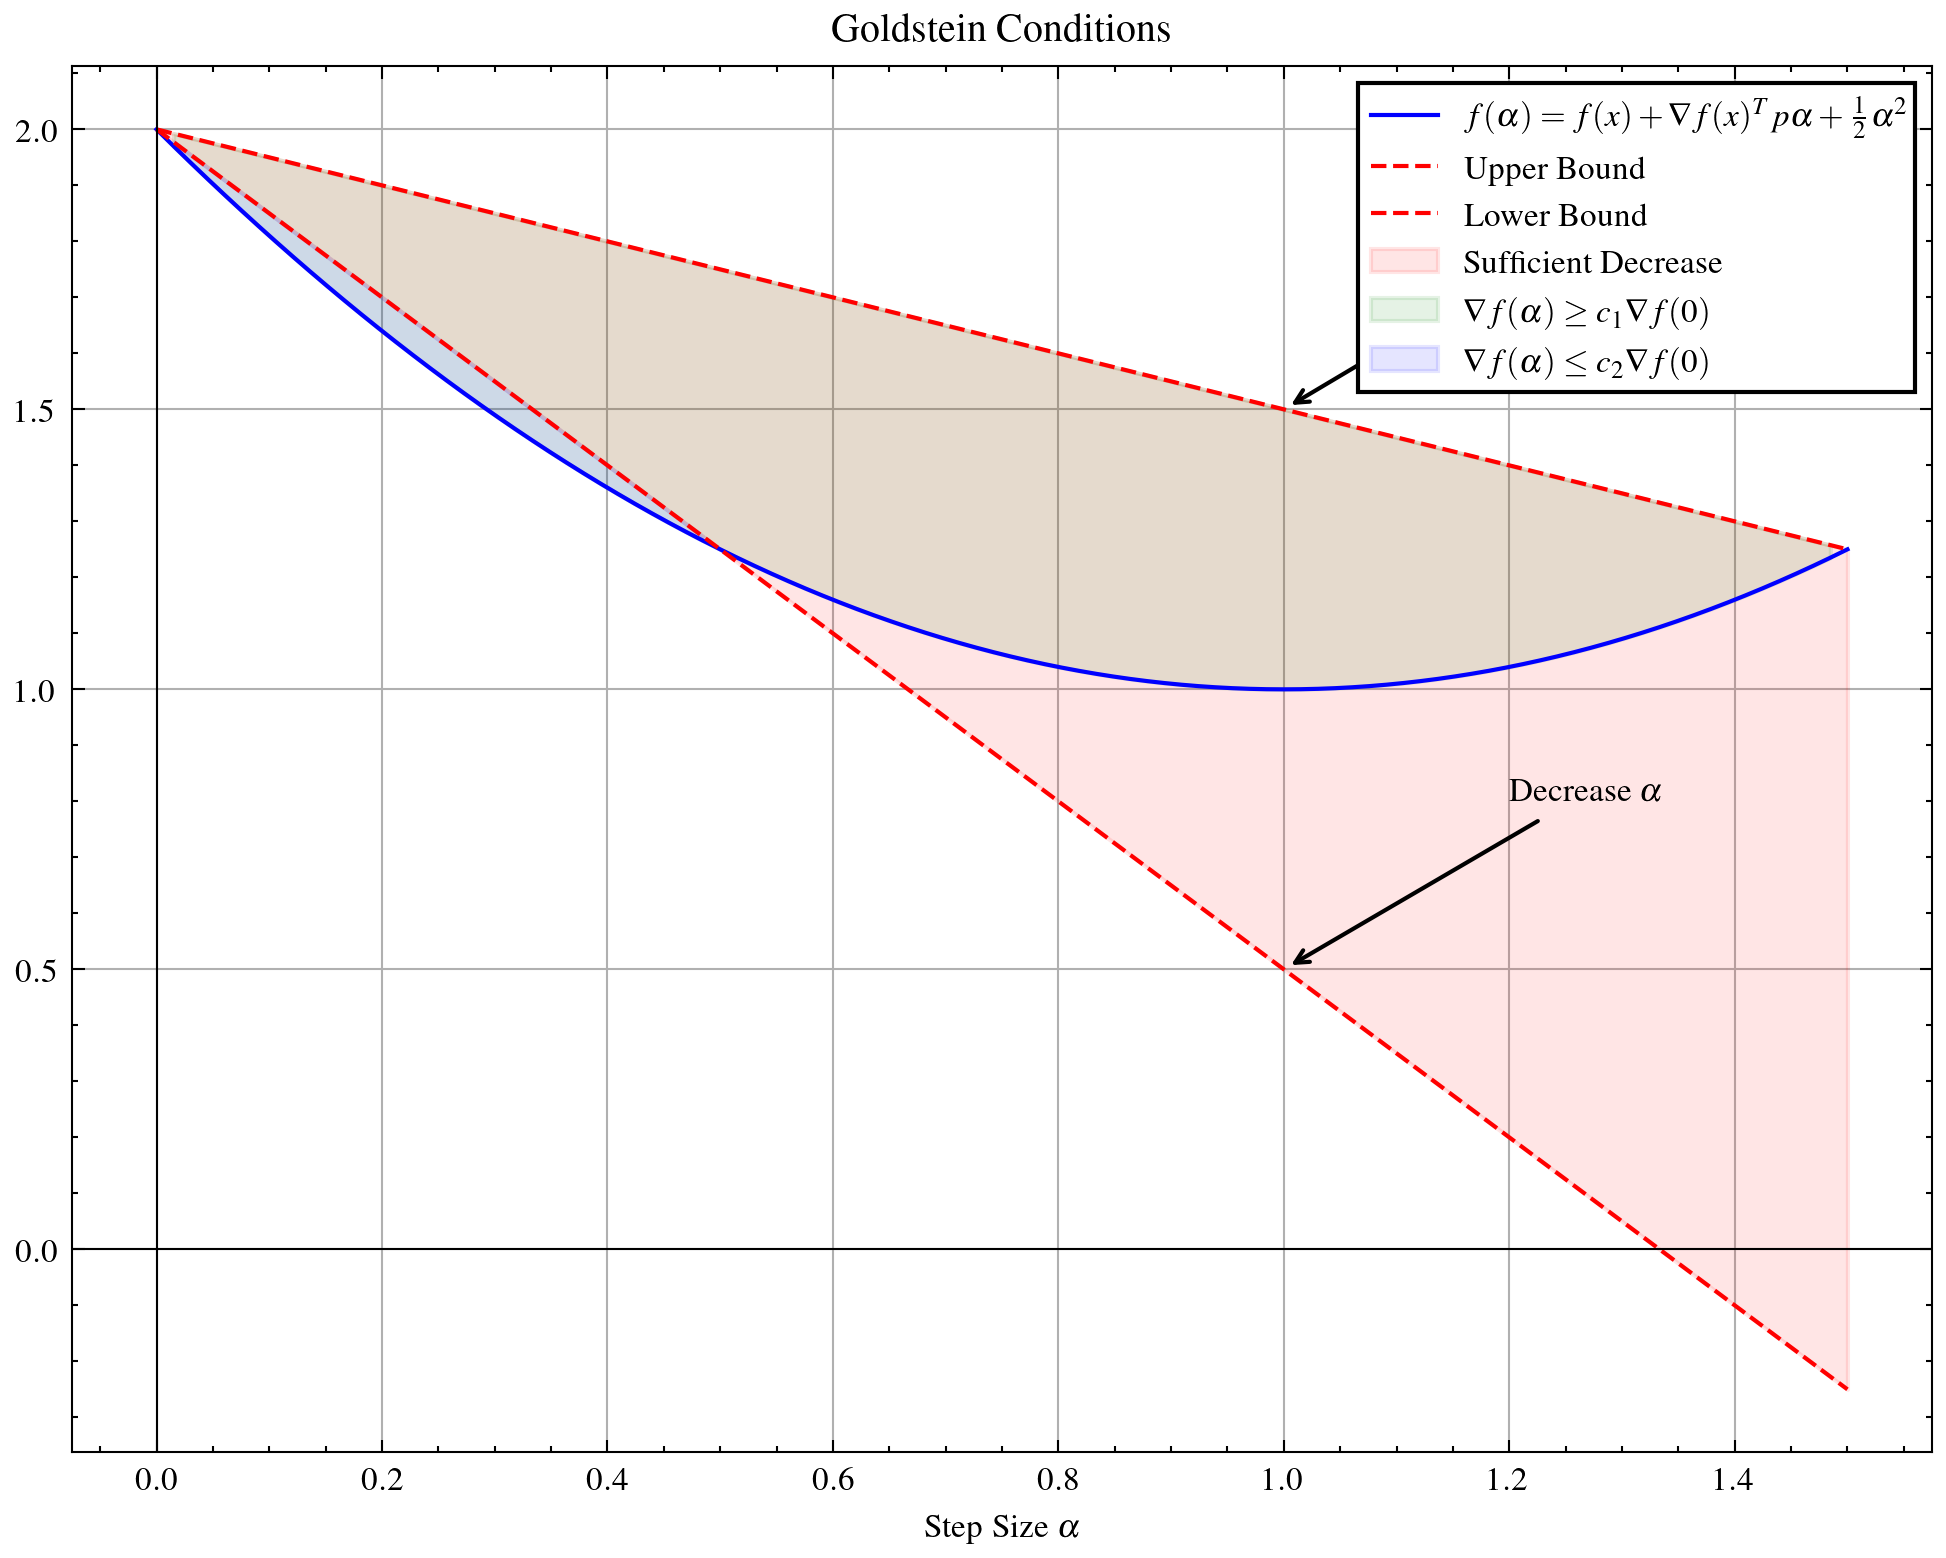
\includegraphics[scale=0.5]{figures/goldstein_conditions.png}
\begin{itemize}
  \item \textbf{Sufficient decrease:}  \(f(x_k + \alpha p_k) \leq f(x_k) + c_1 \alpha \inner{\nabla f(x_k), p_k}\). If this fails, decrease  \(\alpha\) because it is too large.
  \item \textbf{Curvature condition:}  \(f(x_k + \alpha p_k) \geq f(x_k) + c_2 \alpha \inner{\nabla f(x_k), p_k}\). If this fails, increase  \(\alpha\) because it is too small.
  \item Goldstein conditions are more robust than Armijo conditions.
\end{itemize}

\subsubsection*{Wolfe conditions}
Choose  \(0 < c_1 < c_2 < 1\).
\begin{itemize}
  \item \textbf{Sufficient decrease:}  \(f(x_k + \alpha p_k) \leq f(x_k) + c_1 \alpha \inner{\nabla f(x_k), p_k}\). If this fails, decrease  \(\alpha\) because it is too large.
  \item \textbf{Curvature condition:}  \(\inner{\nabla f(x_k + \alpha p_k)}{p_k} \geq c_2 \inner{\nabla f(x_k)}{p_k}\). If this fails, increase  \(\alpha\) because it is too small.
  \item Wolfe conditions are more robust than Goldstein conditions.
\end{itemize}
\subsection{Lecture 6 (24. Januar 2025)}

\section*{Backtracking Linjesøk}
Backtracking Line Search er en metode for å finne en passende skrittlengde \( \alpha \) i iterative optimeringsalgoritmer. Målet er å sikre at skrittet reduserer objektivfunksjonen \( f(\bm{x} + \alpha \bm{p}) \) tilstrekkelig, samtidig som det unngås for små eller ustabile skritt.

\subsection*{Algoritme og Matematisk Formulering}
La \( f: \R^n \to \R \) være kontinuerlig deriverbar, og \( \bm{p} \in \R^n \) en nedstigningsretning (dvs. \( \langle \nabla f(\bm{x}), \bm{p} \rangle < 0 \)). Algoritmen søker \( \alpha > 0 \) som tilfredsstiller \textbf{Armijo-betingelsen}:
\[
  f(\bm{x} + \alpha \bm{p}) \leq f(\bm{x}) + c_1 \alpha \langle \nabla f(\bm{x}), \bm{p} \rangle, \quad c_1 \in (0, 1).
\]

\begin{algorithm}[H]
  \SetAlgoLined
  \DontPrintSemicolon
  \KwIn{ \(\alpha_0 > 0\),  \(c_1 \in (0,1)\),  \(\rho \in (0,1)\)}
  \KwOut{ \(\alpha\)}
  \(\alpha \leftarrow \alpha_0\)\;
  \While{ \(f(\bm{x} + \alpha \bm{p}) > f(\bm{x}) + c_1 \alpha \langle \nabla f(\bm{x}), \bm{p} \rangle\)}{
    \(\alpha \leftarrow \rho \alpha\) \tcp*{Reduser skrittlengde}
  }
  \Return{ \(\alpha\)}
  \caption{Backtracking Linjesøk (Armijo)}
\end{algorithm}

\subsection*{Relaterte Betingelser}
\begin{itemize}
  \item \textbf{Armijo-Goldstein}: Legger til en nedre grense for \( \alpha \):
        \[
          f(\bm{x}) + c_2 \alpha \langle \nabla f(\bm{x}), \bm{p} \rangle \leq f(\bm{x} + \alpha \bm{p}) \leq f(\bm{x}) + c_1 \alpha \langle \nabla f(\bm{x}), \bm{p} \rangle, \quad 0 < c_1 < c_2 < 1.
        \]

  \item \textbf{Wolfe-betingelsene}: Inkluderer krumningstilstand:
        \[
          \langle \nabla f(\bm{x} + \alpha \bm{p}), \bm{p} \rangle \geq c_2 \langle \nabla f(\bm{x}), \bm{p} \rangle, \quad 0 < c_1 < c_2 < 1.
        \]
\end{itemize}

\begin{lemma}{Terminering}{}
  Hvis \( f \in C^2 \) er nedre begrenset og \( \bm{p} \) er en nedstigningsretning, terminerer backtracking-algoritmen med en endelig \( \alpha > 0 \).
\end{lemma}

\begin{theorem}{Konvergens for Gradient Descent}{}
  Anta:
  \begin{itemize}
    \item \( f \in C^2 \) med kompakt nivåmengde \( \mathcal{L}_f(\bm{x}_0) = \{\bm{x} \in \R^n \mid f(\bm{x}) \leq f(\bm{x}_0)\} \)
    \item \( \bm{p}_k = -\nabla f(\bm{x}_k) \)
    \item \( \alpha_k \) tilfredsstiller Armijo- eller Wolfe-betingelsene
  \end{itemize}
  Da gjelder:
  \[
    \lim_{k \to \infty} \|\nabla f(\bm{x}_k)\| = 0.
  \]
\end{theorem}

\begin{example}{Kvadratisk Funksjon}{}
  For \( f(\bm{x}) = \frac{1}{2} \bm{x}^\top Q \bm{x} - \bm{b}^\top \bm{x} \) med \( Q \succ 0 \), gir eksakt linjesøk:
  \begin{align*}
    \alpha_k                          & = -\frac{\langle \bm{p}_k, \nabla f(\bm{x}_k) \rangle}{\langle \bm{p}_k, Q \bm{p}_k \rangle}, \\
    \|\bm{x}_{k+1} - \bm{x}^\star\|_Q & \leq \frac{\kappa - 1}{\kappa + 1} \|\bm{x}_k - \bm{x}^\star\|_Q,
  \end{align*}
  hvor \( \kappa = \operatorname{cond}(Q) = \frac{\lambda_{\max}(Q)}{\lambda_{\min}(Q)} \).
\end{example}

\begin{example}{Rosenbrock-funksjonen: Hessian}{}
  For \( f(x,y) = (1 - x)^2 + 100(y - x^2)^2 \) har Hessianen i minimum \( \bm{x}^\star = (1,1) \) formen:
  \[
    H_f(1,1) = \begin{bmatrix} 802 & -400 \\ -400 & 200 \end{bmatrix}.
  \]
  Kondisjonstallet \( \kappa \approx 2500 \) forklarer treg konvergens for gradientdescent.
\end{example}


\subsection{Lecture 7 (27. Januar 2025)}

\paragraph{Goal for today}
\begin{itemize}
  \item Newton's Method:
        \begin{itemize}
          \item Definition and convergence rate
          \item Combination with line search
          \item Necessary modifications
        \end{itemize}
\end{itemize}

\section*{Newton's Method}

\paragraph{Background}
Assume \(G: \R^d \to \R^d\). We want to solve \(G(x) = 0\).

Newton's method is an iterative procedure for finding the roots of a differentiable function \(G: \R^d \to \R^d\).
It uses the first-order Taylor (linear) approximation of \(G\) at the current point \(x_k\).

\begin{definition}{Newton's Method}{}
  The iteration is defined by
  \begin{align*}
    x_{k+1} & = x_k - \bigl(D G(x_k)\bigr)^{-1} G(x_k),
  \end{align*}
  where \(D G(x_k)\) is the derivative (Jacobian) of \(G\) at \(x_k\). If \(G\) is the gradient of a scalar function \(f\), then \(DG(x_k) = H_f(x_k)\), the Hessian of \(f\).
\end{definition}

\paragraph{Convergence Theory}
If \(G\in \mathcal{C}^2\), then this iteration converges locally \emph{quadratically} to
a solution \(x^\star\) of \(G(x) = 0\), provided that \(D G(x^\star)\) is invertible.

\begin{remark}
  Quadratic convergence means there exist constants \(C>0\) and \(\delta>0\) such that for all \(k\) with \(\|x_k - x^\star\|\le \delta\),
  \[
    \|x_{k+1} - x^\star\| \;\le\; C \,\|x_k - x^\star\|^2.
  \]
\end{remark}

\subsection*{Application to Optimization}

We apply Newton's method to solve \(\nabla f(x) = 0\). That is, to find stationary points of a function \(f:\R^d \to \R\).

\paragraph{Basic Method}
\begin{itemize}
  \item Newton iteration:
        \[
          x_{k+1} \;=\; x_k \;-\; H_f(x_k)^{-1} \,\nabla f(x_k).
        \]
  \item Alternatively, set up the system \(H_f(x_k)\,p_k = -\,\nabla f(x_k)\) and then \(x_{k+1} = x_k + p_k\).
  \item Convergence: If \(f\in \mathcal{C}^3\) and \(H_f(x^\star)\) is nonsingular at the local minimizer \(x^\star\), the method converges locally quadratically.
\end{itemize}

\begin{algorithm}[H]
  \caption{Basic Newton's Method}
  \label{alg:newton-basic}
  \KwInput{Starting point  \(x_0\), tolerance  \(\epsilon > 0\)}
  \KwOutput{Approximate solution  \(x_k\)}
  \(k \gets 0\)\;
  \While{ \(\|\nabla f(x_k)\| > \epsilon\)}{
    Compute Hessian  \(H_f(x_k)\)\;
    Solve  \(H_f(x_k)\,p_k = -\,\nabla f(x_k)\)\;
    \(x_{k+1} \gets x_k + p_k\)\;
    \(k \gets k + 1\)\;
  }
  \KwRet{ \(x_k\)}\;
\end{algorithm}

\paragraph{Global Convergence Strategy}
\begin{enumerate}
  \item Combine with a line search.
  \item Define \(p_k\) by solving \(H_f(x_k)\,p_k = -\nabla f(x_k)\).
  \item Choose a step length \(\alpha_k > 0\).
  \item Update \(x_{k+1} = x_k + \alpha_k \, p_k\).
\end{enumerate}

\begin{algorithm}[H]
  \caption{Globally Convergent Newton's Method}
  \label{alg:newton-global}
  \KwInput{Starting point  \(x_0\), tolerances  \(\epsilon, c > 0\), reduction factor  \(\rho \in (0,1)\)}
  \KwOutput{Approximate solution  \(x_k\)}
  \(k \gets 0\)\;
  \While{ \(\|\nabla f(x_k)\| > \epsilon\)}{
    Compute Hessian  \(H_f(x_k)\)\;
    Solve  \(H_f(x_k)\,p_k = -\nabla f(x_k)\)\;
    \(\alpha_k \gets 1\)\;
    \While{ \(f(x_k + \alpha_k p_k) > f(x_k) + c\,\alpha_k\,\nabla f(x_k)^\top p_k\)}{
      \(\alpha_k \gets \rho\,\alpha_k\)\;
    }
    \(x_{k+1} \gets x_k + \alpha_k p_k\)\;
    \(k \gets k + 1\)\;
  }
  \KwRet{ \(x_k\)}\;
\end{algorithm}

\paragraph{Descent Direction Condition}
If \(H_f(x_k)\) is positive definite, then
\[
  \langle p_k, \nabla f(x_k)\rangle
  \;=\;
  -\,\langle H_f(x_k)^{-1}\,\nabla f(x_k),\,\nabla f(x_k)\rangle
  \;<\; 0,
\]
so \(p_k\) is a descent direction for the line search.

\paragraph{Modified Newton's Method}
If \(H_f(x_k)\) is not positive definite, or if \(\langle \nabla f(x_k), p_k\rangle \geq 0\), then the line search may fail. One approach is to modify the Hessian or switch to a different direction:

\begin{itemize}
  \item First compute \(p_k = -\,H_f(x_k)^{-1}\,\nabla f(x_k)\).
  \item If \(\langle \nabla f(x_k),\,p_k\rangle \;\ge\; \varepsilon \,\|\nabla f(x_k)\|\,\|p_k\|\) for some \(\varepsilon > 0\), switch to \(p_k = -\,\nabla f(x_k)\).
  \item Alternatively, modify the Hessian so it is sufficiently positive definite (e.g.\ shift its eigenvalues).
\end{itemize}

\begin{algorithm}[H]
  \caption{Modified Newton's Method with Hessian Modification}
  \label{alg:newton-modified}
  \KwInput{Starting point  \(x_0\), tolerances  \(\epsilon, \varepsilon > 0\)}
  \KwOutput{Approximate solution  \(x_k\)}
  \(k \gets 0\)\;
  \While{ \(\|\nabla f(x_k)\| > \epsilon\)}{
  Compute Hessian  \(H_f(x_k)\)\;
  Compute eigendecomposition  \(H_f(x_k) = U\,\Lambda\,U^\top\)\;
  \(M \gets \text{diag}\bigl(\max\{\lambda_1, \varepsilon\}, \ldots, \max\{\lambda_d, \varepsilon\}\bigr)\)\;
  \(p_k \gets -\,U\,M^{-1}\,U^\top\,\nabla f(x_k)\)\;
  \uIf{ \(\nabla f(x_k)^\top p_k < -\,\varepsilon\,\|\nabla f(x_k)\|\|p_k\|\)}{
    Use  \(p_k\) as the search direction\;
  }
  \Else{
    \(p_k \gets -\,\nabla f(x_k)\)\;
  }
  % In a global method, we would then do a line search on p_k:
  %   x_{k+1} = x_k + alpha_k p_k
  % but here it is omitted for brevity.
  \(x_{k+1} \gets x_k + p_k\)\;
  \(k \gets k + 1\)\;
  }
  \KwRet{ \(x_k\)}\;
\end{algorithm}

\paragraph{Alternative Interpretation of Newton's Method}
Newton's method can also be viewed via a second-order Taylor expansion of \(f\) around \(x_k\):

\begin{enumerate}
  \item Approximate \(f\) by
        \[
          m_k(p) \;=\; f(x_k) \;+\; \langle \nabla f(x_k),\, p\rangle \;+\; \tfrac12\,\langle H_f(x_k)\,p,\,p\rangle.
        \]
  \item Find \(p_k\) by minimizing \(m_k(p)\).
        \[
          \nabla m_k(p_k) \;=\; \nabla f(x_k) \;+\; H_f(x_k)\,p_k \;=\; 0
          \quad\Longrightarrow\quad
          p_k = -\,H_f(x_k)^{-1}\,\nabla f(x_k).
        \]
  \item If \(H_f(x_k)\) is not positive definite, one modifies it to be positive definite (e.g.\ shifting eigenvalues).
\end{enumerate}

The \emph{modified Newton's method} then reads \(x_{k+1} = x_k + \alpha_k\,p_k\) with \(\alpha_k>0\) found by a line search and \(p_k\) given by one of the strategies above.

\paragraph{Quadratic Convergence Criterion}
Quadratic convergence holds precisely when, near \(x^\star\), we use
\[
  p_k \;=\; -\,H_f(x_k)^{-1}\,\nabla f(x_k)
  \quad\text{and}\quad
  \alpha_k \;=\; 1.
\]
In particular, for \(\alpha_k = 1\) to be acceptable in the line search once \(x_k\) is close to \(x^\star\), the Hessian near \(x^\star\) must be uniformly positive definite (so all eigenvalues \(\ge \varepsilon > 0\)), and the line search parameters (e.g.\ the Armijo or Wolfe constants) must allow a full step.

\section*{Conjugate Gradient Methods}

We now focus on the special case of minimizing the quadratic function
\[
  \Phi(x) \;:=\; \tfrac12\,\langle x,\;Q\,x\rangle \;-\; \langle b,\;x\rangle,
\]
where \(Q \in \R^{d\times d}\) is symmetric positive definite and \(b \in \R^d\). In exact arithmetic, the \emph{Conjugate Gradient} (CG) method can solve this problem in at most \(d\) steps.

With exact line search, the update is
\[
  x_{k+1}
  \;=\; x_k \;-\; \frac{\langle Q\,x_k - b,\;p_k\rangle}{\langle Q\,p_k,\;p_k\rangle}\,p_k,
\]
which ensures
\[
  \langle \nabla \Phi(x_{k+1}),\;p_k\rangle \;=\; 0.
\]
In particular, for a gradient method we would have \(\nabla \Phi(x_{k+1}) \propto p_{k+1}\). Orthogonality conditions arise naturally here.

\paragraph{Conjugate Directions}
A set of vectors \(\{p_0, p_1, \dots, p_{d-1}\}\subset \R^d\) is \emph{conjugate} with respect to \(Q\) if
\[
  \langle p_i,\;Q\,p_j\rangle \;=\; 0 \quad\text{for}\quad i\neq j.
\]
Equivalently, the vectors are mutually orthogonal under the inner product \(\langle u, v \rangle_Q := \langle u, Q\,v\rangle\).

\begin{lemma}{Conjugate Directions}{}
  Let \(\{p_0,\ldots,p_{d-1}\}\) be a conjugate basis of \(\R^d\). Consider the iteration
  \[
    x_{k+1} \;=\; x_k + \alpha_k\,p_k
    \quad\text{with}\quad
    \alpha_k \;=\; -\,\frac{\langle r_k,\;p_k\rangle}{\langle Q\,p_k,\;p_k\rangle},
  \]
  where \(r_k = Q\,x_k - b\). Then \(x_d = x^\star = Q^{-1}b\). In other words, the exact solution is reached in at most \(d\) steps.
\end{lemma}

\begin{proof}{}{}
  Since \(\{p_0,\ldots,p_{d-1}\}\) is a basis, there exist scalars \(\sigma_k\) such that
  \[
    x^\star - x_0
    \;=\; \sum_{k=0}^{d-1} \sigma_k\,p_k.
  \]
  Also,
  \[
    x_d - x_0
    \;=\; \sum_{k=0}^{d-1} \alpha_k\,p_k.
  \]
  To show \(x_d = x^\star\), it suffices to prove \(\sigma_k = \alpha_k\) for all \(k\). Indeed,
  \[
    \sigma_l
    \;=\; \frac{\langle x^\star - x_0,\;Q\,p_l\rangle}{\langle p_l,\;Q\,p_l\rangle}
    \;=\; \frac{\langle Q\,(x^\star - x_0),\;p_l\rangle}{\langle p_l,\;Q\,p_l\rangle}
    \;=\; \frac{\langle b - Q\,x_0,\;p_l\rangle}{\langle p_l,\;Q\,p_l\rangle}.
  \]
  Also,
  \[
    \alpha_l
    \;=\; -\,\frac{\langle r_0,\;p_l\rangle}{\langle Q\,p_l,\;p_l\rangle},
    \quad\text{where}\quad r_0 \;=\; Q\,x_0 - b.
  \]
  Careful manipulation (and using the fact that \(\langle p_i, Q\,p_j\rangle=0\) for \(i\neq j\)) shows \(\sigma_l = \alpha_l\). Hence \(x^\star = x_d\).
\end{proof}

\paragraph{The CG Iteration}
The Conjugate Gradient method constructs a sequence of conjugate directions by choosing
\[
  p_0 = -\,r_0 \;=\; b - Q\,x_0,
  \quad
  p_{k+1} = -\,r_{k+1} + \beta_k\,p_k
\]
with \(\beta_k\) chosen so that \(\langle p_{k+1},\,Q\,p_k\rangle=0\). One can show this leads to convergence in at most \(d\) steps for solving \(Q\,x = b\) in exact arithmetic.

\subsection{Lecture 8 (31. February 2025)}

\textbf{Goals:}
\begin{enumerate}
  \item \textbf{CG Convergence:} Theoretical guarantees and convergence speed
  \item \textbf{Efficient Reformulation:} Practical CG improvements
  \item \textbf{Nonlinear Extension:} Fletcher--Reeves method
  \item \textbf{Step Length Selection:} Optimal step size strategies
  \item \textbf{Alternative Methods:} Polak--Ribière and Hestenes--Stiefel variants
\end{enumerate}

\begin{theorem}{}{}
  As long as \(r_k \neq 0\), we have that:
  \begin{itemize}
    \item \(\inner{r_k, r_e}=0 \forall l = 0,...,k-1 \)
    \item \(\spann\{p_0,\ldots, p_k\} = \spann\{r_0, \ldots, r_k\} = \spann\{r_0, Qr_0, Q^2r_0,\ldots, Q^k r_0\}\)
    \item \(\inner\{p_k, Qp_l\} = 0 \forall \; l=0,\ldots,k-1\)
    \item In particular
  \end{itemize}
\end{theorem}

\begin{lemma}{}{}
  Assume that \(\alpha\) satisfies in each step the strong curvature condition:
  \[
    \left|\inner{}\right|
  \]

\end{lemma}

\subsection{Lecture 9 (3. Februar 2025)}

\begin{definition}{Newton's Method}{newton-method}
  \[
    x_{k+1} = x_k - [\nabla^2 f(x_k)]^{-1} \nabla f(x_k) = x_k - H_k^{-1} \nabla f(x_k) = x_k + p_k
  \]
  where \( H_k \) is the Hessian matrix.
\end{definition}

But computing the Hessian matrix is expensive, so we use the \textbf{quasi-Newton} method instead.

\section*{Quasi-Newton Methods}
The quasi-Newton method is an iterative optimization algorithm that approximates the Hessian matrix using rank-one updates.
This approach avoids the computational cost of computing the exact Hessian matrix and can provide faster convergence rates.
\begin{definition}{Quasi-Newton Method}{quasi-newton}
  \[
    x_{k+1} = x_k - B_k^{-1} \nabla f(x_k) = x_k + p_k
  \]
  where \( B_k \) is an approximation of the Hessian matrix.
\end{definition}

\begin{algorithm}[H]
  \caption{Quasi-Newton Method}
  \label{alg:quasi-newton}
  \SetKwFunction{QuasiNewton}{QuasiNewton}
  \QuasiNewton{ \(x_0\),  \(B_0\),  \(f\),  \(\nabla f\),  \(\epsilon\)}\;
  \While{ \(\norm{\nabla f(x_k)} > \epsilon\)}{
  Compute the search direction  \(p_k = -B_k^{-1} \nabla f(x_k)\)\;
  Choose the step size  \(\alpha_k\) by line search\;
  Update the current point  \(x_{k+1} = x_k + \alpha_k p_k\)\;
  Update the approximation  \(B_{k+1}\) of the Hessian matrix\;
  }
  \KwRet{ \(x_k\)}\;
\end{algorithm}

\paragraph{Update Formulas}

\begin{itemize}
  \item \textbf{DFP update}: \( B_{k+1} = B_k + \frac{y_k y_k^T}{y_k^T s_k} - \frac{B_k s_k s_k^T B_k}{s_k^T B_k s_k} \)
  \item \textbf{BFGS update}: \( B_{k+1} = B_k + \frac{(y_k y_k^T)}{y_k^T s_k} - \frac{(B_k s_k)(B_k s_k)^T}{s_k^T B_k s_k} \)
  \item \textbf{SR1 update}: \( B_{k+1} = B_k + \frac{(y_k - B_k s_k)(y_k - B_k s_k)^T}{(y_k - B_k s_k)^T s_k} \)
  \item \textbf{Broyden update}: \( B_{k+1} = B_k + \frac{(y_k - B_k s_k - B_k^T y_k)(s_k^T B_k)}{s_k^T B_k s_k} \)
\end{itemize}

\subsection*{SR1 Update}
The SR1 update is a rank-one update that approximates the Hessian matrix using the following formula:
\[
  B_{k+1} = B_k + \frac{(y_k - B_k s_k)(y_k - B_k s_k)^T}{(y_k - B_k s_k)^T s_k}
\]
where \( s_k = x_{k+1} - x_k \) and \( y_k = \nabla f(x_{k+1}) - \nabla f(x_k) \).

\clearpage

\subsection{Lecture 10 (7. Februar 2025)}

\paragraph{Læringsmål}
\begin{enumerate}
  \item \textbf{Quasi-Newton Methods}
  \item BFGS
  \item DFP
\end{enumerate}

\paragraph{Fra tidligere: Quasi-Newton Metoder}
\begin{align*}
  p_k     & = -B_k^{-1} \nabla f(x_k) = -H_k^{-1} \nabla f(x_k) \\
  x_{k+1} & = x_k + \alpha_k p_k                                \\
  B_{k+1} & = B_k + \text{update}
\end{align*}

\paragraph{DFP oppdatering: Regne ut \(B_{k+1}\)}
\begin{itemize}
  \item \textbf{Symmetrisk}
  \item \textbf{Sekantligning}: \(B_{k+1} s_k = y_k\) med \(s_k = x_{k+1} - x_k\) og \(y_k = \nabla f(x_{k+1}) - \nabla f(x_k)\).
  \item \(B_{k+1}\) er nærme \(B_k\) og tilfredsstiller sekantligningen.
\end{itemize}

Nytt: tolk "nærme" som minimeringen av en norm.

Definer \( B_{k+1} \) som løsning til
\[
  \min_{B \in \R^{d \times d}} \frac{1}{2} \norm{B - B_k}_F^2 \quad \text{s.a.} \quad B = B^T, \quad B s_k = y_k
\]

Valg av norm: Frobeniusnormen
\[
  G := \int_0^1 H_f(x_k + \tau \alpha p_k) \, d\tau
\]
Definerer en form for gjennomsnittlig Hessian av \( f \) langs linjen \([x_k, x_{k+1}]\).

La \( W = G^{-1} \) (der \( G \) er invertibel).

Definerer \( \norm{A}_W = \norm{WA}_F = \sqrt{\sum_{i,j} (W A)_{ij}^2} \).

\begin{remark}{}{}
  \begin{align*}
    Gs_k & = G(x_{k+1} - x_k) = G(\alpha p_k)                                                                                                                 \\
         & = \int_0^1 \overbrace{H_f(x_k + \tau \alpha p_k) \alpha p_k}^{\frac{\partial}{\partial \tau}\left[\nabla f(x_k + \tau \alpha p_k)\right]} \, d\tau \\
         & = \nabla f(x_k + \alpha p_k) - \nabla f(x_k) = y_k \quad \implies \quad Gs_k = y_k \quad \text{og} \quad W y_k = s_k
  \end{align*}
\end{remark}

\begin{theorem}{}{}
  Assume \(W\in \R^{d \times d}\) is symmetric positive definite, non-singular, and \(W y_k = s_k\). Then the solution to
  \[
    \min_{B \in \R^{d \times d}} \frac{1}{2} \norm{B - B_k}_W^2 \quad \text{s.a.} \quad B = B^T, \quad B s_k = y_k
  \]
  is given by
  \[
    B_{k+1} = \left(I - \rho_k y_k \otimes s_k\right) B_k \left(I - \rho_k s_k \otimes y_k\right) + \rho_k y_k \otimes y_k
  \]
  where \( \rho_k = \frac{1}{\inner{y_k, s_k}} \).

  This is the Davidon-Fletcher-Powell method (DFP).
\end{theorem}

\hrule
\vspace{1em}

\paragraph{BFGS oppdatering (Broyden-Fletcher-Goldfarb-Shanno)}

One can again work with \(H_k = B_k^{-1}\) instead.
Here we obtain the update formula:
\[
  H_{k+1} = H_k - \frac{\left(H_k y_k\right) \otimes \left(H_k y_k\right)}{\inner{y_k, H_k y_k}} + \frac{s_k \otimes s_k}{\inner{y_k, s_k}}
  = H_k + \frac{(s_k - H_k y_k)(s_k - H_k y_k)^T}{\inner{y_k, s_k}}
\]

Alternativt kan vi starte direkte med \(H_k \):

Definerer \( H_{k+1} \) med å minimere \( \norm{H - H_k}_G \) s.a. \( H = H^T \) og \( H y_k = s_k \).
Da får vi Broyden-Fletcher-Goldfarb-Shanno (BFGS) metoden.

\[
  H_{k+1} = H_k + \left(I - \rho_k s_k \otimes y_k\right) \left(I - \rho_k y_k \otimes s_k\right) + \rho_k s_k \otimes s_k \quad \text{med} \quad \rho_k = \frac{1}{\inner{s_k, y_k}}
\]

\begin{lemma}{}{}
  Anta at \( H_k \) er positiv definit og kan finnes med \textit{BFGS} eller \textit{DFP} oppdateringer.
  Hvis \( \inner{y_k, s_k} > 0 \), så er \( H_{k+1} \) positiv definit.
\end{lemma}

\begin{proof}{BFGS}{}
  La \( z \in \R^d \backslash \{0\} \) være en vilkårlig vektor.
  Da er:
  \begin{align*}
    \inner{z, H_{k+1} z} & = \inner{z, H_k z} + \inner{z, \left(I - \rho_k s_k \otimes y_k\right)H_k \left(I - \rho_k y_k \otimes s_k\right) z} + \rho_k \inner{z, \left(s_k \otimes s_k\right) z}   \\
                         & = \inner{\overbrace{\left(I - \rho_k y_k \otimes s_k\right) z}^{w}, H_k \overbrace{\left(I - \rho_k s_k \otimes y_k\right) z}^{w}} + \rho_k \inner{z, \inner{s_k, z} s_k} \\
                         & = \inner{w, H_k w} + \rho_k \inner{s_k, z}^2 \geq 0 \quad \text{og} \quad \inner{z, H_{k+1} z} = 0 \iff \inner{s_k, z} = 0, \quad w = 0
  \end{align*}
  Nå er \( w = \left(I - \rho_k y_k \otimes s_k\right) z = z - \rho_k \inner{y_k, z} s_k \), så hvis \( \inner{s_k, z} = 0 \) så er \( w = z \neq 0 \).
  Dermed er enten \( \rho_k\inner{y_k, z}^2\) eller \( \inner{w, H_k w} \) positiv, så \(\implies H_{k+1} \) er positiv definit.
  
  \qed
\end{proof}


Hvis vi kan garantere at \( \inner{y_k, s_k} \gg 0 \; \forall k \) og \( H_0 \) er positiv definit, så vil \( H_{k+1} \) være positiv definit for alle \( k \), og \(p_{k+1} = -H_{k+1} \nabla f(x_k) \) vil være en nedstigningsretning.

Hvis \( f \) er strengt konveks\ref{def:rem:strictly_convex} ( og dermed \(x_{k+1} \neq x_k \) for alle \( k \)), så vil 
\[
\inner{\nabla f(x_{k+1}) - \nabla f(x_k), x_{k+1} - x_k} > 0
\]

\begin{itemize}
  \item Anta at \(\alpha_k\) er valgt mhp Wolfe-betingelsene. Da er
  \[
    \inner{\nabla f(x_k + \alpha_k p_k), p_k} \geq c_2 \inner{\nabla f(x_k), p_k} \quad \text{og} \quad \inner{\nabla f(x_{k+1}), p_k} \geq c_1 \inner{\nabla f(x_k), p_k}
  \]
  \item Implementer BFGS/DFP oppdateringene med linjesøk (Wolfe-betingelsene) og velg \( H_0 \) positiv definit.
  \[
    H_0 = c \, I \quad \text{hvor} \quad c > 0
  \]

  \item Vanlig strategi: I første steg velg \( p_0 = -\nabla f(x_0) \) og finn \( \alpha_0 \) med linjesøk (f.eks. Wolfe-betingelsene).
  \item Deretter finner vi \(x_1 = x_0 + \alpha_0 p_0 \) og \( s_0 = x_1 - x_0 \) og \( y_0 = \nabla f(x_1) - \nabla f(x_0) \).
  \item Definerer så \( c = \frac{\inner{y_0, s_0}}{\inner{y_0, y_0}} \) og \( H_0 = c \, I \).
  \item Regn ut \( H_1 = H_0 + \text{BFGS/DFP update} \).
\end{itemize}

\begin{figure}[H]
  \begin{minipage}[t]{0.49\textwidth}
    \begin{algorithm}[H]
      \caption{BFGS with Wolfe Conditions} 
      \label{alg:bfgs}
      \KwIn{Initial point \(x_0\), tolerance \(\epsilon>0\), \(N\), \(H_0 = I\)}
      \For{\(k=0,1,\ldots,N\)}{
        Compute \(g_k = \nabla f(x_k)\)\;
        \If{\(\|g_k\| < \epsilon\)}{
          \Return{\(x_k\)}\;
        }
        Set \(p_k = -H_k g_k\)\;
        Find step size \(\alpha_k\) via Wolfe line search\;
        Update \(x_{k+1} = x_k + \alpha_k p_k\)\;
        Set \(s_k = x_{k+1} - x_k\)\;
        Set \(y_k = \nabla f(x_{k+1}) - g_k\)\;
        Set \(\rho_k = \frac{1}{y_k^\top s_k}\)\;
        Update inverse Hessian:
        \[
          H_{k+1} = (I - \rho_k s_k y_k^\top) H_k (I - \rho_k y_k s_k^\top) + \rho_k s_k s_k^\top
        \]
      }
      \Return{\(x_{k+1}\)}\;
    \end{algorithm}
  \end{minipage}
  \hfill
  \begin{minipage}[t]{0.49\textwidth}
    \begin{algorithm}[H]
      \caption{DFP with Wolfe Conditions}
      \label{alg:dfp}
      \KwIn{Initial point \(x_0\), tolerance \(\epsilon>0\), \(N\), \(B_0 = I\)}
      \For{\(k=0,1,\ldots,N\)}{
        Compute \(g_k = \nabla f(x_k)\)\;
        \If{\(\|g_k\| < \epsilon\)}{
          \Return{\(x_k\)}\;
        }
        Solve \(B_k p_k = -g_k\) for \(p_k\)\;
        Find step size \(\alpha_k\) via Wolfe line search\;
        Update \(x_{k+1} = x_k + \alpha_k p_k\)\;
        Set \(s_k = x_{k+1} - x_k\)\;
        Set \(y_k = \nabla f(x_{k+1}) - g_k\)\;
        Set \(\rho_k = \frac{1}{y_k^\top s_k}\)\;
        Update Hessian: \(B_{k+1} = (I - \rho_k y_k s_k^\top) B_k (I - \rho_k s_k y_k^\top) + \rho_k y_k y_k^\top\)
      }
      \Return{\(x_{k+1}\)}\;
    \end{algorithm}
  \end{minipage}
\end{figure}
